%%%%%%%%%%%%%%%%%%%%%%%%%%%%%%%%%%%%%%%%%
% University/School Laboratory Report
% LaTeX Template
% Version 3.1 (25/3/14)
%
% This template has been downloaded from:
% http://www.LaTeXTemplates.com
%
% Original author:
% Linux and Unix Users Group at Virginia Tech Wiki 
% (https://vtluug.org/wiki/Example_LaTeX_chem_lab_report)
%
% License:
% CC BY-NC-SA 3.0 (http://creativecommons.org/licenses/by-nc-sa/3.0/)
%
%%%%%%%%%%%%%%%%%%%%%%%%%%%%%%%%%%%%%%%%%

%----------------------------------------------------------------------------------------
%	PACKAGES AND DOCUMENT CONFIGURATIONS
%----------------------------------------------------------------------------------------

\documentclass{article}

\usepackage[version=3]{mhchem} % Package for chemical equation typesetting
\usepackage{siunitx} % Provides the \SI{}{} and \si{} command for typesetting SI units
\usepackage{graphicx} % Required for the inclusion of images
\usepackage{natbib} % Required to change bibliography style to APA
\usepackage{amsmath} % Required for some math elements 
\usepackage[colorlinks,linkcolor=blue ]{hyperref}

\usepackage{listings}
\usepackage{xcolor}

    \definecolor{mygreen}{rgb}{0,0.6,0}  
    \definecolor{mygray}{rgb}{0.5,0.5,0.5}  
    \definecolor{mymauve}{rgb}{0.58,0,0.82} 
    \lstset{ %  
      backgroundcolor=\color{white},   % choose the background color; you must add \usepackage{color} or \usepackage{xcolor}  
      basicstyle=\footnotesize,        % the size of the fonts that are used for the code  
      breakatwhitespace=false,         % sets if automatic breaks should only happen at whitespace  
      breaklines=true,                 % sets automatic line breaking  
      captionpos=bl,                    % sets the caption-position to bottom  
      commentstyle=\color{mygreen},    % comment style  
      deletekeywords={...},            % if you want to delete keywords from the given language  
      escapeinside={\%*}{*)},          % if you want to add LaTeX within your code  
      extendedchars=true,              % lets you use non-ASCII characters; for 8-bits encodings only, does not work with UTF-8  
      frame=single,                    % adds a frame around the code  
      keepspaces=true,                 % keeps spaces in text, useful for keeping indentation of code (possibly needs columns=flexible)  
      keywordstyle=\color{blue},       % keyword style  
      %language=Python,                 % the language of the code  
      morekeywords={*,...},            % if you want to add more keywords to the set  
      numbers=left,                    % where to put the line-numbers; possible values are (none, left, right)  
      numbersep=5pt,                   % how far the line-numbers are from the code  
      numberstyle=\tiny\color{mygray}, % the style that is used for the line-numbers  
      rulecolor=\color{black},         % if not set, the frame-color may be changed on line-breaks within not-black text (e.g. comments (green here))  
      showspaces=false,                % show spaces everywhere adding particular underscores; it overrides 'showstringspaces'  
      showstringspaces=false,          % underline spaces within strings only  
      showtabs=false,                  % show tabs within strings adding particular underscores  
      stepnumber=1,                    % the step between two line-numbers. If it's 1, each line will be numbered  
      stringstyle=\color{orange},     % string literal style  
      tabsize=1,                       % sets default tabsize to 2 spaces  
      %title=myPython.py                   % show the filename of files included with \lstinputlisting; also try caption instead of title  
    }  

\setlength\parindent{0pt} % Removes all indentation from paragraphs

\renewcommand{\labelenumi}{\alph{enumi}.} % Make numbering in the enumerate environment by letter rather than number (e.g. section 6)

%\usepackage{times} % Uncomment to use the Times New Roman font

%----------------------------------------------------------------------------------------
%	DOCUMENT INFORMATION
%----------------------------------------------------------------------------------------

\title{Projects of Compiler Principles \\ CS215} % Title

\author{Yaoming \textsc{Zhu}} % Author name

\date{5140219355} % Date for the report

\begin{document}



\maketitle % Insert the title, author and date

\begin{center}
\begin{tabular}{l r}
Date Performed: & January 18, 2017 \\ % Date the experiment was performed

Instructor: & Professor Li Jiang % Instructor/supervisor
\end{tabular}
\end{center}

% If you wish to include an abstract, uncomment the lines below
% \begin{abstract}
% Abstract text
% \end{abstract}

%----------------------------------------------------------------------------------------
%	SECTION 1
%----------------------------------------------------------------------------------------

\section{Objective}

In this project, it is required to design and implement a simplified compiler, for a given programming language, namely smallC, which can be regarded as a subset and the core part of C programming language. The complier should translate smallC source code to MIPS assembly codes. 

% If you have more than one objective, uncomment the below:
%\begin{description}
%\item[First Objective] \hfill \\
%Objective 1 text
%\item[Second Objective] \hfill \\
%Objective 2 text
%\end{description}

\subsection{Project Logic}
\label{definitions}
\begin{description}
\item[Lexical Analyzer]  The \textit{Flex} tool is used to help design a lexical analyzer generator.
\item[Syntax Analyzer]   The \textit{Bison}(A.K.A \textit{Yacc}) tool is used to help design an LALR parser generator. 
\item[Abstract Syntax Tree] After syntax analysis, the AST tree can be generated. It helps to test the output of former process. 
\item[Semantic Analyzer] Possible semantic errors is checked in this part.
\item[Intermediate Representation Code Translation] The AST tree is translated into IR code in this part.
\item[Optimization] Some optimizations are applied to IR code in this part, i.e. dead code elimination.
\item[Machine-code Generation] The IR code is interpreted into MIPS code in this part.
\item[Project Test] Test the project with some smallC code and SPIM.
\end{description} 

\subsection{Project Environment}
The project guidance says "In this project, Linux environment (Ubuntu) is required". Fortunately, with the help of \textit{bash on ubuntu on windows}, this project can be implemented under Windows system. 

Furthermore,  
\textit{Win flex-bison} provided with all flex and bison function to the Windows platform, which means this project can be implemented even under Windows IDE! (And I actually finished most parts of the project with Visual Studio 2015). With IDE support, the debugging process becomes much more efficient and precise.

For setup details, please refer to \\
 \url{https://sourceforge.net/p/winflexbison/wiki/Visual%20Studio%20custom%20build%20rules/}

\begin{figure}[h]
\begin{center}
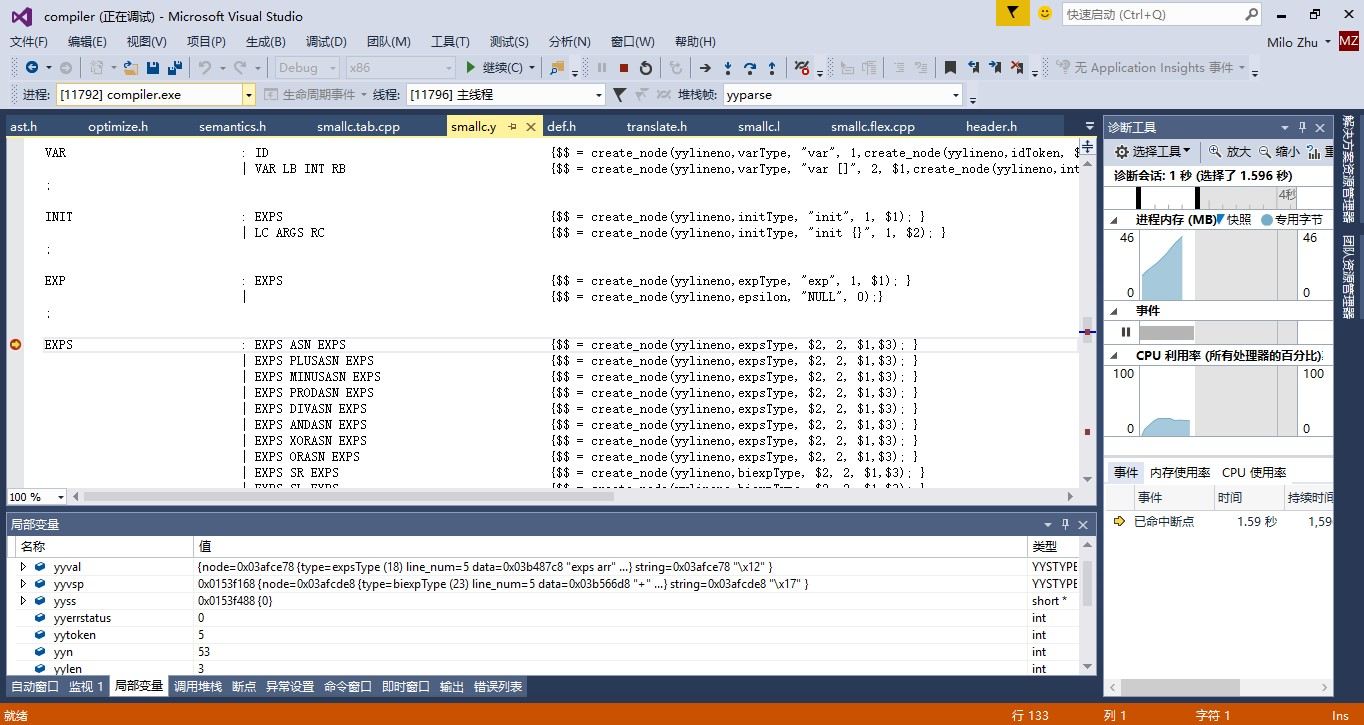
\includegraphics[width=1\textwidth]{IDE.jpg} % Include the image placeholder.png
\caption{The Project on Visual Studio 2015}
\end{center}
\end{figure}

Besides the FTP-uploaded one, I have also uploaded a Visual Studio project, they only small difference they have is that, for the output short name of \textit{Win flex-bison} is different form Ubuntu one, thus it leads to different head file reference. You can access Visual Studio version form the link in readMe file.

%----------------------------------------------------------------------------------------
%	SECTION 2
%----------------------------------------------------------------------------------------

\section{Lexical Analyzer}

With the help of \textit{Flex}, this part is fairly simple. 

This part is done in \textit{smallC.l}.

\subsection{Keywords}
Since the keywords are fixed, the lexical analyzer will return corresponding token and string value once it find the keywords. \emph{yylval} is provided by \textit{flex} to help to capture the string content of our token. 

\begin{lstlisting}[language = C] 
int												{yylval.string = strdup(yytext); return TYPE;}
struct											{yylval.string = strdup(yytext); return STRUCT;}
return											{yylval.string = strdup(yytext); return RETURN;}
if												{yylval.string = strdup(yytext); return IF;}
else											{yylval.string = strdup(yytext); return ELSE;}
break											{yylval.string = strdup(yytext); return BREAK;}
continue										{yylval.string = strdup(yytext); return CONT;}
for												{yylval.string = strdup(yytext); return FOR;}
read											{yylval.string = strdup(yytext); return READ;}
write											{yylval.string = strdup(yytext); return WRITE;}
\end{lstlisting}

\emph{Note.} According to the guidance, the \emph{'read'} and \emph{'write'} are not the smallC keywords. However, they are used to test input and output function the compiler, thus they are regarded as keywords in this project. 

\subsection{Numbers and Identifiers}
The token for numbers and identifiers are a little more tricky, regular expression is needed. 

\begin{lstlisting}[language = C] 
digitnon0 [1-9]
hexdigit [0-9A-Fa-f]
letter [A-Za-z]
digit  ({digitnon0}|0)

identifier ((_|{letter})(_|{letter}|{digit})*)
dec_int  (({digitnon0})+({digit})*)
oct_int  (0({digit})*)
hex_int  (0(x|X)({digit})*)
%%
....// keywords
{dec_int}											{yylval.string = strdup(yytext); return INT; }
{oct_int}											{yylval.string = strdup(yytext); return INT; }
{hex_int}											{yylval.string = strdup(yytext); return INT; }
{identifier}										{yylval.string = strdup(yytext); return ID;}
\end{lstlisting}

\subsection{Blank Characters and Comments}
Like most C-like languages, smallC will just ignore the blank characters, so do the lexical analyzer. The only exception is the newline characters: the lexical analyzer will use it to get current line number. A variable \textit{yylineno} is introduced to keep record of current line number. 

\begin{lstlisting}[language = C] 
extern int yylineno;

%%
[\t\r\f]											{;}
[\n]												{yylineno++;}
[ ]													{;}

\end{lstlisting}

As for comments, two different cases shall be treated, the in-line comment(//) and the out-of-line comment(/* */). The former one will end once the newline character is encountered, the later one will end only if "*/" is encountered. 

\begin{lstlisting}[language = C] 

void commentInLine();
void commentOutLine();

%%
"//"				{commentInLine();}
"/*"				{commentOutLine();}
%%

void commentInLine(void){
	char c;
	while((c = input())!='\n');
	yylineno++;
}

void commentOutLine(void){
	char c1, c2;
	c2 = input();
	do{
		c1 = c2;
		c2 = input();
		if(c1 == '\n'){
			yylineno++;		
		}
	}while(!(c1 == '*' && c2 == '/'));
}
\end{lstlisting}

\subsection{Test}

Unless otherwise specified, the following smallC code will be used as test code. 

\begin{lstlisting}[language = C,title={test.c}] 
int main()
{
	int x;
	read(x);
	x = x + 10;
	write(x);
	return 0;
}
\end{lstlisting}

After \textit{flex} the .l file and compile, we can get the result:

\begin{figure}[h]
\begin{center}
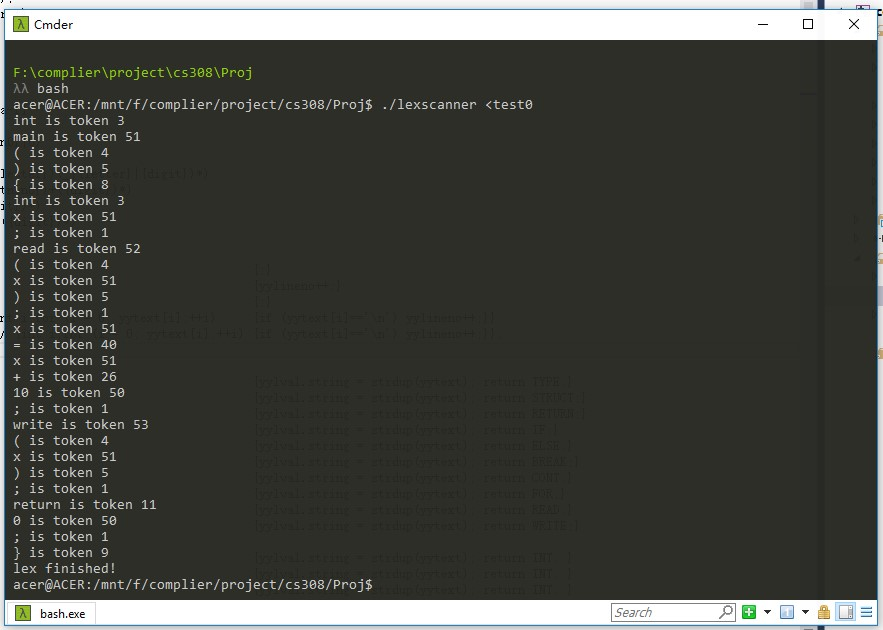
\includegraphics[width=1\textwidth]{Lex.jpg} % Include the image placeholder.png
\caption{The Output of Lexical Analyzer}
\end{center}
\end{figure}

The lexical analyzer works well.

%----------------------------------------------------------------------------------------
%	SECTION 3
%----------------------------------------------------------------------------------------

\section{Syntax Analyzer}

The design of syntax analyzer is simple but tough.

This part is done in \textit{smallC.y}. \textit{Bison} is used in this part.

First and foremost, a data structure is required to represent abstract syntax tree(AST). Thus, a struct is constructed as AST node, which shall have following functions:
\begin{enumerate}
\item Hold the AST node type
\item Hold the pointers pointing to its sub AST-node.
\end{enumerate}

Thus, it is designed as:

\begin{lstlisting}[language = C] 
typedef struct TreeNode {
    nodeTypeEnum type;
    int lineNum;
    char* data;
    int size, capacity;
    struct TreeNode** children;
} TreeNode;
\end{lstlisting}
\textit{size} and \textit{capacity} hold values for number of this kind of AST node and max number of AST can have respectively. \textit{lineNum} is the corresponding line number of the AST node.
\textit{data} store some informations. For terminals(i.e. identifier), it contains string content; for non-terminals, it store the derivation case, for most non-terminals have more than one production.
\textit{type} is an enum type to hold the AST node type, which is defined as 
\begin{lstlisting}[language = C] 
typedef enum{
	programType,
	extdefsType,
	extdefType,
	//......other non-terminals
	unaryopType,
	idToken,
	biexpType,
	keywords,
	typeToken,
	intToken,
	epsilon
} nodeTypeEnum;
\end{lstlisting}
Besides the non-terminals given by the guidance, here some other AST types are introduced:
\begin{enumerate}
\item
Terminal types: keywords, typeToken, intToken, idToken,epsilon
\item
Auxiliaries: unaryopType, biexpType
\end{enumerate}

"Auxiliaries" is special cases of \textit{EXPS} non-terminal. \textit{unaryopType} is for unary operators, while \textit{biexpType} is for all binary expressions other than those concerned with assignment.

Since the sub AST varies from AST node types, a variable arguments functions is implemented to create AST node in the process.

\begin{lstlisting}[language = C] 
TreeNode* createNode(int lineno,nodeTypeEnum type, char* data, int cnt, ...) {
    TreeNode* ptr = (TreeNode*)malloc(sizeof(TreeNode));
    ptr->lineNum = lineno;
    ptr->type = type;
    ptr->data = strdup(data);
    ptr->size = ptr->capacity = cnt;
    ptr->children = (TreeNode**)malloc(sizeof(TreeNode*) * cnt);
    va_list ap;
    va_start(ap, cnt);
    int i;
    for (i = 0; i < cnt; i++) {
        ptr->children[i] = va_arg(ap, TreeNode*);
    }
    va_end(ap);
    return ptr;
}
\end{lstlisting}

Then, the grammars of smallC is translated into \textit{bison} file. Taken \textit{EXTDEF} as instance:

\begin{lstlisting}[language = C] 
EXTDEF						: TYPE EXTVARS SEMI							{$$ = createNode(yylineno,extdefType, "extdef1", 2, createNode(yylineno,typeToken, $1, 0),$2); }
							| STSPEC SEXTVARS SEMI						{$$ = createNode(yylineno,extdefType, "extdef2", 2, $1,$2); }
							| TYPE FUNC STMTBLOCK						{$$ = createNode(yylineno,extdefType, "extdef func", 3, createNode(yylineno,typeToken, $1, 0),$2,$3); }
;
\end{lstlisting}

As the guidance indicated, grammar given may induce one or two reduce-reduce/shift-reduce conflicts. Specifically, \textit{"IF LP EXP RP STMT”} should have lower precedence than \textit{“IF LP EXP RP STMT
ELSE STMT”}. A trick of \textit{bison} is applied here:


\begin{lstlisting}[language = C] 
%nonassoc LOWER_THAN_ELSE
%nonassoc ELSE
%%
STMT:		//......
							| IF LP EXPS RP STMT %prec IFX				{$$ = createNode(yylineno,stmtType, "if stmt", 2, $3,$5); }
							| IF LP EXPS RP STMT ELSE STMT %prec ELSE	{$$ = createNode(yylineno,stmtType, "if stmt", 3, $3,$5,$7);}
 ;
\end{lstlisting}

One more modification is applied to grammar. As \textit{read} and \textit{write} is regarded as keywords in the project, the production of \textit{STMT} now is 
\begin{lstlisting}[language = C] 
STMT						: EXP SEMI									{$$ = ...; }
							| STMTBLOCK									{$$ = ...; }
							| RETURN EXPS SEMI							{$$ = ...; }
							| IF LP EXPS RP STMT %prec IFX				{$$ = ...; }
							| IF LP EXPS RP STMT ELSE STMT %prec ELSE	{$$ = ...;}
							| FOR LP EXP SEMI EXP SEMI EXP RP STMT		{$$ = ...; }
							| CONT SEMI									{$$ = ...; }
							| BREAK SEMI								{$$ = ...; }
							| READ LP EXPS RP SEMI						{$$ = ...;}
							| WRITE LP EXPS RP SEMI						{$$ = ...;}
\end{lstlisting}

%----------------------------------------------------------------------------------------
%	SECTION 4
%----------------------------------------------------------------------------------------

\section{Abstract Syntax Tree}

This part is done in \textit{ast.h} and \textit{def.h}. 

With \textit{samllC.y} finished, the program now can output the AST. The struct \textit{TreeNode} has already implemented the tree, thus the generation of AST is quite simple with techniques learned form data structure classes.
\begin{lstlisting}[language = C] 
void printAst(TreeNode* ptr, int depth) {
    int i;
    int n = (depth - 1) * 2;
    
    if (depth > 0) {
        for (i = 0; i < n; i++) {
            putchar(buffer[i]);
        }
        putchar('|');
        puts("");
    }
    
    for (i = 0; i < n; i++) {
        putchar(buffer[i]);
    }
    if (depth > 0) {
        putchar('|');
        putchar('_');
    }
    n = depth * 2;
    buffer[n] = '|';
    buffer[n + 1] = ' ';
	if (ptr == NULL) {
		printf("NULL\n");
		return;
	}
    printf("%s\n", ptr->data);
    // terminal customized configuration
    if (ptr->size > 0) {
        printf("%s\n", ptr->data);
    } else {
        printf("%s\n", ptr->data);
        
        for (i = 0; i < n; i++) {
            putchar(buffer[i]);
        }
        puts("");
        
    }
    for (i = 0; i < ptr->size; i++) {
        if (i == ptr->size - 1) {
            buffer[n] = ' ';
        }
        printAst(ptr->children[i], depth + 1);
    }
}
\end{lstlisting}

The AST of test.c is stored at file \textit{AST}. It turned out that the syntax analyzer works well.


%----------------------------------------------------------------------------------------
%	SECTION 5
%----------------------------------------------------------------------------------------

\section{semantic analysis}

This part is done in \textit{semantic.h}.

In this part, potential semantic errors after generating a parse tree is checked. Besides, the symbol table is generated. Some basic evaluation (i.e. get values of int) is also done in this part.


\subsection{Symbol Table}
In this part, a struct is designed to implement the symbol table. 
\begin{lstlisting}[language = C] 
struct ptr_cmp {
	bool operator()(const char* s1, const char* s2) const {
		return strcmp(s1,s2) < 0;
	}
};
struct SymbolTable {
	map <char*, char*,ptr_cmp> table;
	map <char*, vector<char *>, ptr_cmp > struct_table;
	map <char*, vector<char *>, ptr_cmp > struct_id_table;
	map < char*, int, ptr_cmp > struct_name_width_table;
        map <char*, int, ptr_cmp> width_table; 
	map <char*, vector<int>, ptr_cmp> array_size_table;
	int parent_index;
} symTable[MAX_LEVEL][MAX_DEPTH];
\end{lstlisting}
Here STL data structure \textit{map} is used for string-key inquiry. 

As the member variable name indicates, they are used to map between:

\begin{table}[!hbp]
    \begin{tabular}{|l|l|l|}
\hline
    member                       & string & key                                                    \\ 
\hline
    table                       & local/global variable names & variable's type                                                    \\ \hline
    struct\_table               & struct names                & all member variable names of the struct            \\ \hline
    struct\_id\_table           & struct names                & member names certain type of the struct \\ \hline
    struct \_name\_width\_table & struct names                & the number of members of the struct                                \\ \hline
    width\_table                & int/array names             & space it comsumes                                                  \\ \hline
    array\_size\_table          & array names                 & vhow many 4 bytes of the width each dimension \\ \hline
    \end{tabular}
    \caption{Symbol Table Content}
\end{table}

\textit{symTable[MAX\_LEVEL][MAX\_DEPTH]}: Here the symbol table is implemented as 2D array. The row index indicates the level of certain table. The smallC code has code blocks("{ }"), which requires a new symbol table. when the program is running, the symbol table of each code blocks has its own scope. Thus it is necessary to keep the level on track. 

Besides, member variable \textit{parent\_index} is used to record the upper level's index.  \textit{parent\_index} will be 1 for global symbol table.

\subsection{Semantic Checking}
For each AST node type, a corresponding check function is implemented.Normally it will get the AST node type of its sub-AST and call corresponding check function to check its sub-tree one by one. i.e.
\begin{lstlisting}[language = C] 
void check_program(TreeNode* p) {
	if (p == NULL) return;
	int i;
	for (i = 0; i < p->size; ++i) {
		check(p->children[i]);
	}
}
\end{lstlisting}

Specifically, the following things need to be checked: (since the amount of code in this part is really large, only design logic instead of code is presented here)

\subsubsection{Variables and functions should be declared before usage}
For variables, every time an identifier node is encountered, the compiler will check it in the symbol table on current level and its upper levels.

For functions, the complier only allows global functions, which is checked on level 0 symbol table. \textit{Overloaded function} is allowed in the compiler, thus not only the function name but its arguments will be checked in this part. 

\subsubsection{Variables and functions should not be redeclared}
Similarly to the previous one, whenever a new variable is declared, it will be checked in the current-level symbol table to find out whether it has already existed.

\subsubsection{Reserved words can not be used as identifiers}
Whenever an identifier node is encountered, its name(stored in the \textit{data}) will be compared to keywords.

\subsubsection{Program must contain a function int main() to be the entrance}
A global variable \textit{bool\_main} is initialized to be false. Once \textit{main} is detected in \textit{FUNC} node, it will be true,otherwise the semantic checking won't pass.

\subsubsection{The number and type of variable(s) passed should match the definition of the function}
This part is already done as a by-product of part 5.2.1

\subsubsection{Use [] operator to a non-array variable is not allowed}

With \textit{width\_table} from symbol table, the compiler can get access to the space an array or variable consumes. From it the compiler can tell whether it is an array or a int, then [] operation to int will be rejected.

\textit{Note.} The declaration like a[1] is not allowed by the compiler, since it cannot distinguish it with ordinary int.

\subsubsection{The . operator can only be used to a struct variable}
With \textit{struct\_table} from symbol table, the complier can check whether a variable has been declared as struct. Then with \textit{struct\_id\_table}, the identifier after . is checked whether it is a member of the struct.

\subsubsection{\textit{break} and \textit{continue} can only be used in a \textit{for}-loop}
A global bool variable is declared to tell whether the current \textit{STMT} node is inside a loop.

\subsubsection{Right-value can not be assigned by any value or expression}
This part will be implemented in the intermediate representation section.

\subsubsection{The condition of if statement should be an expression with int type}
The logic is similar to part 5.2.6, \textit{width\_table} is checked to tell the type of expression. 

\subsubsection{The condition of for should be an expression with int type or epsilon}

\subsubsection{Only expression with type int can be involved in arithmetic}
These parts are similar to 5.2.10

\subsubsection{Other details}
\begin{enumerate}
\item
Size of array can’t be negative or 0
\item
Members of a struct and argument of a function can’t have same names
\end{enumerate}


%----------------------------------------------------------------------------------------
%	SECTION 6
%----------------------------------------------------------------------------------------

\section{Intermediate Representation Code Translation}

This part is done in \textit{translate.h}. 

Here comes the most tough, complex and exhausting part. 
After passing semantic analysis, the smallC code can be regarded as a correct one and the AST node will be translated into intermediate representation(IR).


\subsection{Intermediate Representation}
Here a MIPS-like three-address code is selected as IR. The different between IR and MIPS is IR has infinite registers so that every variable can be hold in the registers. 

Like before, a struct is designed to implement IR instructions.

\begin{lstlisting}[language = C] 
// for MIPS generation
struct Address{
    RegType type; //type of the argument
    string name; //For labels and function calls
    int value; // register value
    int real;// physical register in MIPS
    int needload; // whether load op is necessary
    int needclear;//  whether this op should be cleared
};

struct Quadruple{
    string op; // name of operation
    int active; //whether it's active
    int flag; //whether its arguments should be modified
    Address arguments[3]; //the three arguments 
};
\end{lstlisting}

RegType in struct Address is an enum type, which represent the type of corresponding address. It can be:
\begin{enumerate}
\item
ADDRESS\_LABEL: The address is jump label number
\item
ADDRESS\_CONSTANT: The address is constant number
\item
ADDRESS\_TEMP: It represents a register
\item
ADDRESS\_NAME: It represents a name
\end{enumerate}

\begin{table}[!h]
    \begin{tabular}{|l|l|l|l|l|}
    \hline
    opname & Destination &  			Operand 1        &  			Operand 2 & Description                  \\ \hline
    or     & a           & b                    & c             & $a = b|c    $                  \\ \hline
    xor    & a           & b                    & c             & a = b\^c                     \\ \hline
    and    & a           & b                    & c             & a = b\&c                    \\ \hline
    sll    & a           & b                    & c             & $a = b<<c    $                 \\ \hline
    srl    & a           & b                    & c             & $a = b>>c     $                \\ \hline
    add    & a           & b                    & c             & $a = b+c     $                 \\ \hline
    sub    & a           & b                    & c             & $a = b-c$                      \\ \hline
    mul    & a           & b                    & c             & $a = b*c  $                    \\ \hline
    div    & a           & b                    & c             & $a = b/c $                     \\ \hline
    rem    & a           & b                    & c             &$ a = b\%c  $                   \\ \hline
    neg    & a           & ~                    & ~             &$ a = -b   $                    \\ \hline
    lnot   & a           & b                    & ~             & $a = !b   $                    \\ \hline
    not    & a           & b                    & ~             & $a = ~b   $                   \\ \hline
    beqz   & ~           & a                    & label         & if a==0 goto label           \\ \hline
    bnez   & ~           & a                    & label         & if a!=0 goto label           \\ \hline
    bgez   & ~           & a                    & label         & if a>=0 goto label           \\ \hline
    bgtz   & ~           & a                    & label         & if a>0 goto label            \\ \hline
    blez   & ~           & a                    & label         & if a<=0 goto label           \\ \hline
    bltz   & ~           & a                    & label         & if a<0 goto label            \\ \hline
    li     & a           & b(constant)          & ~             & a = b                        \\ \hline
    lw     & a           & b                    & c(constant)   & a = mem[b+c]                 \\ \hline
    sw     & [memory]    & a,b,c(c is constant) & ~             & mem[b+c] = a                 \\ \hline
    move   & a           & b                    & c             & a = b                        \\ \hline
    label  & ~           & l                    & ~             & l is int, set label          \\ \hline
    goto   & ~           & l                    & ~             & l is int, unconditional jump \\ \hline
    func   & ~           & s                    & ~             & s is string, set function    \\ \hline
    call   & ~           & s                    & ~             & s is string, call function   \\ \hline
    \end{tabular}
    \caption{Three Address Code Logic}
\end{table}

Some vectors are also used to help the translation process:
\begin{lstlisting}[language = C] 
vector <Quadruple> IR, GIR, MIR;
vector <int> RegisterState, RegisterOffset,LabelCont, LabelBreak, vs_reg; 
vector <string> vs_id;
\end{lstlisting}

\begin{enumerate}
\item
RegisterState: The register can either hold value or address. RegisterState is used to tell its current state
\item
RegisterOffset: contains the info of offsets of the register.
\item
LabelBreak and LabelCont: indicates the label for break and continue operation.
\item
vs\_reg and vs\_id:  associates identifiers with the registers.
\end{enumerate}

\subsection{Translate}
\subsubsection{EXPS translate}
For \textit{EXPS} AST ndoe, the complier will classify it into following cases:


\begin{description}
\item[Arithmetic] A new register will be allocated to store the result of the arithmetic process
\item[Logical] The following IR is used to assign the bool value to register:
\begin{lstlisting} 
li [register],1
beqz/bnez/bgez/bgtz/blez/bltz judgement label
li [register],0
label 1
\end{lstlisting}
\item[Unary] 
For ordinary ones, a new register will be allocated.

For "++" and "--", not only a new register is allocated but the one participating in the operation will be modified as well.

\item[Assignment] First, the operations like "*=" will be decomposed into arithmetic one and pure assignment.

Then for pure assignment, the compiler will just do register modifications.

\item[Array and Struct] Offset will be applied to visit the member.
\end{description}

\subsubsection{FUNC translate}
The arguments of functions are stored on the stack. 

Every time a function(except main()) call is encountered, the \$ra will be stored in the stack. The stack pointer will be restalled after function call. 

\subsubsection{STMT translate}

\begin{description}
\item[if] \textit{goto} label in IR can be used here. That is if the judgement of if is false, the complier will use jump to else statement(let's call it s2); otherwise it will first execute the statement right after judgement(let's call it s1). Then a \textit{goto} is placed right after s1 to jump out of the block, which will not execute s2 in the case.

\item[for] \textit{goto} label in IR can be used here, too. The basic logic is almost the same except there are one more jump label to jump back in order to form a loop. 
 
\item[read and write]
\end{description} The \textit{read()} is to assign the value of register \$v0 into the register associated with variable, while \textit{write()} assign value to register \$a0. 

It is implemented with \textit{scanf\_one} and \textit{printf\_one}

\begin{lstlisting} 
__printf_one:
li $v0, 1
syscall
jr $ra
__scanf_one:
li $v0,5
syscall
jr $ra
\end{lstlisting}




\section{Optimization}
Subexpression elimination and dead code elimination is done in this part. 
\subsection{Subexpression elimination}
This part is done in \textit{optimize.h}

Subexpression elimination are like change:
\begin{lstlisting} 
move t2,t1
move t3,t2
\end{lstlisting}
into
\begin{lstlisting} 
move t3,t1
\end{lstlisting}
and
\begin{lstlisting} 
li t1,1
move t2,t1
\end{lstlisting}
into
\begin{lstlisting} 
move t2,1
\end{lstlisting}

Here t2 must not be reassigned afterwards.
A flag is used to indicate whether the register is reassigned later. 


\subsection{Instruction Selection}
This part is done in \textit{interprete.h}

The following operation is done to reinforcement optimization:

\begin{enumerate}
\item
Check labels and delete those whose destination immediately following.

\item
For all arithmetic expressions, interpret into intermediate instructions. 

\item
Check for successive lws and sws. Delete the sw where the the former instruction is lw and their target are the same. 

\item
use shift operations when multiplying 2 or 4.

\end{enumerate}

\section{Machine Code Generation}
This part is done in \textit{interprete.h} and \textit{optimize.h}

After optimization, the compiler will interpret the IR into MIPS code. The major difference between IR and MIPS is the number of registers. Thus the compiler shall implement register allocation.

Here the compiler will scan through \$11 to \$25 to find out the free register. If no free one, it will scan \$8 to \$10. If no register is available currently, \textit{lw} and \textit{sw} will be applied to store variables into memory. 

\subsection{Project Test}
The complier is already finished, the test is necessary. 

The test.c is translated into 
\begin{lstlisting}][title={MIPS.s}] 
.globl main

.data
temp: .space 44

.text
__printf_one:
li $v0, 1
syscall
jr $ra
__scanf_one:
li $v0,5
syscall
jr $ra

main:
la $a3, temp
add $11, $29, -40
move $13, $11
move $11, $13
jal __scanf_one
sw $2, 0($11)
move $11, $13
move $12, $13
lw $12, 0($12)
add $12, $12, 10
sw $12, 0($11)
move $11, $13
lw $11, 0($11)
move $4, $11
jal __printf_one
li $11, 0
add $12, $29, 4
sw $11, 0($12)
j __program_end
j __program_end
__program_end:
li $v0, 10
syscall

\end{lstlisting}
\begin{figure}[h]
\begin{center}
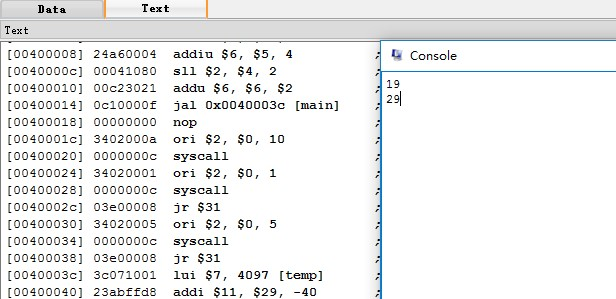
\includegraphics[width=1\textwidth]{SPIM.jpg} % Include the image placeholder.png
\caption{Test on SPIM}
\end{center}
\end{figure}
It runs on QtSPIM precisely. The compiler works well.

\section{Acknowledgement}

This project is large and tough. After finishing it, I learned a lot about compliers ,C language and MIPS. 

I would like to express my sincere thanks to instructor Prof. Jiang and teaching assistant. The class and project taught me a lot. Thank you for your contribution!



%----------------------------------------------------------------------------------------
%	BIBLIOGRAPHY
%----------------------------------------------------------------------------------------

\bibliographystyle{apalike}

\bibliography{sample}

%----------------------------------------------------------------------------------------


\end{document}